\section{DUNE Data Characteristics}
\label{sec:data-characteristics}
\subsection{Overview}

A number of parameters from DUNE/LBNF requirements, design documents,  and studies are used  as input
for estimations of the data rates in DUNE.
%In cases when derived parameters need to be generated based on these inputs this is accomplished using
%the software package \textit{dune-params}\cite{duneparams}
%developed specifically for this purpose. As the inputs and estimations are refined the results presented in this annex can be regenerated at will.
Buffering, triggering and readout strategy and algorithms of the DAQ
are complex R\&D items and are far from their final design and state of
readiness at the time of writing. Same applies to various analysis software.
For that reason, the data rate estimations involve some broad assumptions
and leave open some choices. This is described in more detail in the following subsections.

DUNE contains a number of major detector subsystems. The Far Detetor (FD) Liquid Argon TPC will present most
challenges from the standoint of real-time data processing and triggering, and can potentially dominate the data volume.
It incorporates the Photon Detector (PD) which while important produces less data so it won't be our focus
for the purpose of the data rate and volume estimates. There are also Near
Detector (ND) Systems (see~\ref{sec:nds-params}) which are complex and for which most data metrics are yet to be developed
at the time of writing.

\subsection{DUNE Detectors and Subsystems}

\subsubsection{Fundamental Parameters of the Far Detector LArTPC}
\label{sec:fundamental-parameters}

The fundamental TPC parameters most relevant as input to the data rate estimations are summarized in
table~\ref{tab:fundamental-parameters}.

\begin{table}[ht!]
	\centering
	\begin{tabular}{| p{2.5in} | p{1in} |}
		\hline
		\textbf{Parameter} & \textbf{Value} \\ \hline
		Full height (single module) & 12.0\,m \\ \hline
		Full width (single module) & 14.5\,m \\ \hline
		Full length (single module) & 58.0\,m \\ \hline
		\# of detector modules & 4 \\ \hline
		\hline
		channels per APA & 2,560 \\ \hline
		APAs per module & 150 \\ \hline
		Active height (APA) & 6.0\,m \\ \hline
		Active width (APA) & 2.3\,m \\ \hline  \hline
		Drift distance in Liquid Argon & 3.6\.m \\
		\hline
		Drift velocity & 1.6\,mm/$\mu$s \\ \hline
		Drift time & 2.25\,ms \\ \hline
		\# drifts/readout factor & 2.4 \\ \hline
		readout time & 5.4\,ms \\ \hline \hline
		bytes/sample & 1.5 \\ \hline
		sample rate & 2.0\,MHz \\ \hline
		samples/readout & 10,800 \\
		\hline \hline
		Total \# of channels & 1,536,000 \\
		\hline
	\end{tabular}
	\caption{Fundamental parameters of DUNE Far Detector LArTPC.}
	\label{tab:fundamental-parameters}
\end{table}

Two of the parameters listed above (``drifts/readout'' and ``readout time'') need an additional comment.
The nominal readout time of 5.4ms is chosen such that additional time windows are covered just before and just
after the nominal $t_0$ (trigger) window. The value of 5.4\,ms is 2.4 times larger than the nominal drift of 2.25\,ms,
and it's listed in the table as the ``drifts/readout'' factor. This factor is not calculated precisely but was chosen based
on the experience with the 35t prototype (Sec.\ref{sec:35t}). The motivation behind this exta readout it to capture
potential activity in the TPC just before and just after the event of interest, so as to characterize this extraneous
ionization which for example can manifest itself as track segments due to cosmic rays background. It is quite
possible that the readout time will be revised as the final detector design is progressing, however the value of 5.4\,ms
was fixed in this document as nominal, in order to provide consistency of various estimates related to the data.

\subsubsection{The Photon Detector}
\label{sec:pd}
The Photon Detector (PD) which is built into the Far Detector LArTPC takes advantage of the fact that Liquid Argon
is an excellent scintillating medium.
The most significant requirements for the PD include determination of $t_0$ of an event relative to the TPC timing ---
resolution better than 1\,$\mu$s (event position resolution along drift direction of a few mm), and sufficient light
collection efficiency to allow triggering on neutrinos coming from a supernova, with the capability of detecting neutrinos with energies as
low as 20\,MeV.

Light produced by Liquid Argon Stintillation is collected from the TPC volume by the wavelength shifter and transported
by the light guide to the Silicon Photo-Multiplier (SiPMs) mounted at its end. A single whole assembly is mounted on each  APA frame.
The SiPMs are read out using shielded twisted-pair cables and the signal is passed to the module called SSP (the SiPM Signal
Processor). Digitized data is processed by a  Field-Programmable Gate Array (FPGA). The use
of the FPGA processing allows for a significant amount of customization of the SSP operation.


\subsubsection{The Near Detector Systems}
\label{sec:nds-params}
For sake of brevity, only basic information will be provided for the Near Detector Systems (NDS) which are under active development
at the time of writing and for which there is no final design yet. The main NDS components are:
\begin{itemize}
\item Near neutrino detector (NND), and its major component, the Fine-Grained Tracker
\item Beamline Measurement System (BLM)
\end{itemize}
\ 
In the reference design at the time of writing, the Fine-Grained Tracker (FGT) near consists of a straw-tube
tracking detector (STT), $\mu$-identifiers (MuID) and electromagnetic calorimeter (ECAL), all placed inside of a 0.4\,T dipole magnet.

\begin{table}[ht!]
\centering
\begin{tabular}{| p{2in} | p{1.5in} |}		\hline		
\textbf{Item} & \textbf{Specification} \\ \hline
Straw Tube Geometry & $\diameter$1\,cm$\times$3.5\,m length \\ \hline
Number of straw tubes & 107,520\\ \hline
Straw tubes per plane & 336 \\ \hline
Planes per module & 4 \\ \hline
Number of modules & 80 \\ \hline
Number of channels & 215,040 \\ \hline
\end{tabular}
\caption{Main parameters of the FGT}
\label{tab:fgt-params}
\end{table}

The FGT is designed to make precision measurements of the neutrino
fluxes, cross sections, signal and background rates at the percent level. A summary of basic parameters of the
NDS are presented in Table~\ref{tab:nds-params}.
\begin{table}[ht!]
\centering
\begin{tabular}{| p{1in} | p{1in} | p{1in} |}		\hline		
\textbf{Detector} & \textbf{Mass} & \textbf{Channels} \\ \hline
SST & 8t & 215,040 \\ \hline
ECAL & 93t & 52,224 \\ \hline
MuID & 100t & 165,888 \\ \hline
\end{tabular}
\caption{Main parameters of the Near Detector Systems}
\label{tab:nds-params}
\end{table}

The Beamline Measurement System (BLM) will be located in the region of the Absorber Complex
at the downstream end of the decay region to measure the muon fluxes from hadron decay.
It is not anticipated to produce large amounts of data when compared to other detectors in DUNE.

\subsection{The Far Detector LArTPC Data}
\label{sec:fd-data-overview}
\subsubsection{Sources of Data in the FD TPC}

Data being read out from the FD TPC are the result of a few different classes of interactions and other phenomena,
as outlined in table~\ref{tab:dune-data-sources}. Characteristics of these sources will
be a major factor influencing the rate and volume of data produced in DUNE.
\begin{table}[ht!]
	\centering
	\begin{tabular}{| p{1in} | p{4.5in} |}
		\hline
	\textbf{Type} & \textbf{Description} \\ \hline
		
	in-spill & Any activity in the detector which is coincident with
	the passage of beam neutrinos through the detector \\ \hline
	
	with-beam-$\nu$ & A subset of \textit{in-spill} where activity is
	consistent with a beam-$\nu$ interacting in the detector \\ \hline
	
	cosmic-$\mu$ & Activity due to the passing of cosmic-ray muons
	through the detector \\ \hline
	
	radioactivity & Activity due to the decay of radioactive
	isotopes \\ \hline
	
	atm-$\nu$ & Activity consistent with interactions from
	atmospheric neutrinos \\ \hline
	
	noise & Electronics noise (common-mode not considered) \\ \hline

	\end{tabular}
	\caption{Sources of data in the LArTPC.}
	\label{tab:dune-data-sources}
\end{table}

Not included in this table are two of the more exotic sources of signal, the Supernova Burst and Nucleon decay.
Due to their rare (and generally speaking, potential) occurance and differing characeristics they will be considered separately
in~\ref{sec:snb-data} and \ref{sec:pdk-data}.

\subsubsection{Segments of the Dynamic Range of the TPC signals}

Signals produced by individual wires in the DUNE TPC will have a substantial
dynamic range. For example, $\beta$-decay of naturally occurring isotope $^{39}$Ar has the endpoint of
565\,keV, whereas signals due to interactions of energetic neutrinos can produce signals
equivalent up to a few MeV energy deposition in a given channel depending on the event topology.

Each segment of the dynamic range will reflect certain types of events and this
be characterized by a respective data rate. For a systematic approach to estimates
and to reflect the physics of the detector, it is helpful to consider three such segments when characterizing the LArTPC data.
To set the scale for these segments we can assign ``thresholds''corresponding to each of them.
The threshold values can be applied to signals on ``per-wire'' basis and defined for example
in terms of ADC values (reflecting the collected charge, which can be translated to units like MeV with proper calibration).
These are not meant to be precise values used in data collection and are given here for orientation purposes only.
Using this concept the dynamic range can be considered with three distinct settings:
\begin{description}
	
\item[full-stream] The full-stream \textbf{(FS)} threshold means \textit{there is no threshold at all}, i.e.
FS data is effectively read out in every time bin (as defined by the ADC clock) and from every channel.

\item[zero-suppressed] The zero-suppression \textbf{(ZS)} threshold is an ADC value (in a single time bin,
on a single wire) roughly corresponding to ionization charge due to a 0.5\,MeV energy deposition.
All bins with ADC counts below this threshold are discarded from the data stream.

\item[high-energy] A high-energy \textbf{(HE)} threshold is assumed to be high enough so that
  that all electronics noise signals from radioactive decays are suppressed but low
  enough to not impact activity from beam neutrino interactions or potential nucleon decay activity.
  Further studies are needed to determine this threshold but currently
  it is taken, without rigor, to be $O(1)$\,MeV.

\end{description}

The categories thus introduced will be considered in more details in the following sections, for example
see \ref{sec:zs-data} for a discussion of Zero Suppression and \ref{sec:ar39decays} for a discussion of
$^{39}$Ar decays rejection.


\subsubsection{Full-stream Data}

Full-stream (FS) data corresponds to reading all data in every ADC channel without
application of any threshold. Estimating the corresponding rate is a calculation based on
known parameters as it does not depend on the activity in the detector or the noise
level of the electronics. As its name implies, it is the most voluminous type of data
that can be generated by the TPC. The parameters which apply to this data are given in
table~\ref{tab:full-stream-parameters}.

\begin{table}[ht!]
	\centering
	\begin{tabular}{| p{3in} | p{1.1in} |}
		\hline

	\textbf{Parameter} & \textbf{Value} \\ \hline
	
	Bytes per sample & 1.5 \\ \hline
	
	DAQ sample rate & 2.0\,Mhz \\ \hline
	
	Channels per APA & 2,560 \\ \hline
	
	Number of APA per detector module & 150 \\ \hline
	
	Number of modules & 4 \\ \hline
	
	Total channels in DUNE & 1,536,000 \\ \hline \hline
	
	Drifts per readout & 2.4 \\ \hline
	
	Drift time & 2.25\,ms \\ \hline

	Total readout window & 5.4\,ms \\ \hline \hline
	
	Beam spill repetition rate & 0.83\,Hz \\ \hline
	
	Annual run time fraction & 0.667 \\ \hline
	\end{tabular}
	\caption{Parameters pertaining to full-stream data rates.}
	\label{tab:full-stream-parameters}
\end{table}
The expected data rates for FS data are given
in table~\ref{tab:full-stream-volume}.
\begin{table}[ht!]
	\centering
	\begin{tabular}{| p{3in} | p{1.1in} |}
		\hline	
	
	\textbf{Parameter} & \textbf{Value} \\ \hline
	Full-stream readout size & 24.9\,GB \\ \hline
	Full-stream 1 year in-spill data volume & 436\,PB \\ \hline
	Full-stream 1 second data volume & 4.6\,TB \\
	Full-stream 1 minute data volume & 276.5\,TB \\	\hline
	Full-stream 1 year data volume & 145.4\,EB \\ \hline
	\end{tabular}
	\caption{Data volumes and rates for full-stream data acquisition.}
	\label{tab:full-stream-volume}
\end{table}
The first row gives the data size corresponding to one DAQ readout cycle (5.4\,ms, as explained in \ref{sec:fundamental-parameters}).
The second is appropriate for any strategy that intends to record FS data for each beam spill.
The third contains two numbers that characterize data volume relevant to a strategy which aims
to record FS data for Supernova Burst candidates. The final row  shows the total annual data
volume that the DUNE DAQ is capable of producing (purely in theory).
\textit{These numbers are not meant to imply ongoing recording of full-stream
data to permanent storage} and are only given to better define the problem and initial parameters
of recording data in DUNE.


\subsubsection{Potential capabilities of the Far Detector TPC DAQ system}
\label{sec:daq-assumptions}
For more detail on the DUNE Data Acquisition see Section~\ref{sec:daq}. One of its central components
is an array of \textit{Reconfigurable Cluster Elements} (RCE)~\cite{slac_rce_1}, which offer very high
readout speeds, considerable real-time computing power and flexibility of system configuration.

In addition to considerations of various signal sources, the data rate estimates depend on capabilities of the DAQ system,
in particular as they apply to data compression and rejection of radiological background.
Examples of relevant DAQ capabilities to be considered are:

\begin{itemize}

\item Identification by the DAQ trigger farm of small and scattered regions of isolated activity
  consistent with $^{39}$Ar decays in order to suppress these data.

\item Ability of the RCEs to apply zero suppression algorithms
with a given threshold to real-time data sent to the trigger farm.

\item Trigger-specific zero suppression algorithms and thresholds to be applied
in the RCEs to the data sent to the data farm.

\item Possibility of RCE-local data storage (e.g. to serve as a buffer for near-time SNB trigger decision).

\item Detection of Regions of Interest (ROI) for high-threshold events, e.g. identifying the APAs
which register the signal of an energetic lepton resulting from a beam neutrino interaction, so as
to avoid collecting and writing the data from ``empty'' parts of each TPC module.

\end{itemize}

\noindent
Based on the current understanding of progress in DAQ R\&D, it is reasonable to expect at the time of
writing that the above DAQ characteristics will indeed be implemented in DUNE.




\subsubsection{Zero-Suppressed Data}
\label{sec:zs-data}
The Far Detector LArTPC is expected to operate is very low background conditions. In practice
is means that in each instance the signals of interest (such as induced by reactions of beam neutrinos)
will only present in a fraction of channels. There are options in choosing the exact zero-suppression (ZS)
procedure, and the final choice has not been made. The simplest procedure may be implemented
as follows: in each channel, all digitized time bins in which the ADC values are below the given threshold
are removed. More discussion on possible alternative ZS methods and their impact on the data rate are given below.

For purposes of this discussion, the nominal ZS threshold is set to be the ADC counts equivalent to 0.5\,MeV energy deposited
as ionization which is collected by a single wire. It is assumed that the application of zero-suppression at this
threshold completely removes ADC counts due to just noise. % although an estimate of data rates due to noise is given.
Estimations of different sources of ZS data are summarized in Table~\ref{tab:zs-volume}.

In order to better preserve the shape of the signal waveform digitized and recorded for
each channel, a more complex strategy may be applied where the data is accepted in additional
time windows before and after the ``main'' pulse which exceeds the nominal ZS threshold. This
is a subject of R\&D at the time of writing. Obviously, implementation of such scheme will lead
to an increase in the recorded data volume compared to the minimalistic version. Assuming that
each extra window is comparable in duration to the peak of the signal above the threshold,
a rough estimate is that this factor could be on the scale of a factor of 2 or 3. However, given
that the design of this and other compression algorithms is still ongoing, and for better consistency
and ease of reference, this is not included in the ZS data estimates presented Table~\ref{tab:zs-volume}.
	
\begin{table}[ht!]
\centering
\begin{tabular}{| p{1.2in} | p{0.9in} | p{0.75in} | p{0.8in} | p{0.9in} |}		\hline		
Source & Event Rate & Event Size & Data Rate & Volume/year \\ \hline
all $^{39}$Ar & 11.2\,MHz & 150\,B & 1.6 GB/s &  53\,PB \\ \hline
all in-spill & & & & 159\,TB \\ \hline
with-beam-$\nu$ & & & & 79\,GB \\ \hline \hline
cosmic-$\mu$ & 0.259\,Hz &2.5\,MB & 647.4\,kB/s & 20\,TB \\	\hline
beam-$\nu$ & 8770\,year$^{-1}$ & 2.5\,MB & 0.69 kB/s & 22 GB \\ \hline \hline
SNB cand. (ZS) & 12 year$^{-1}$ & 16.7\,GB & 6366\,B/s & 201\,GB \\ \hline
SNB cand. (FS) & 12 year$^{-1}$ & 46.1\,TB & 17.5\,MB/s & 553\,TB \\ \hline
\end{tabular}
\caption{Data rate estimations for ZS data from various sources.
An additional FS data estimation is given for the Supernova Burst (SNB).}
\label{tab:zs-volume}
\end{table}

One other factor that must be considered in any discussion or implementation of ZS is the data design,
i.e. the method and format by which the sparse zero-suppressed data is packaged and included into
data stream and put into storage. As some examples show (see~\ref{sec:data-compression})
there can be gross inefficiencies in the data format due to implicit dependencies
on software components and algorithms used in the applications handling these data.
Numbers shown in Table~\ref{tab:zs-volume} for cosmic-$\mu$ and beam-$\nu$
are therefore a known overestimation. They are presented as they reflect the status
of a few software components at the time creation of the DUNE Conceptual Design Report,
however the final numbers will be revised downward in \ref{sec:fd-data-volume-summary}
before inclusion into the Computing Model.

\subsubsection{Atmospheric $\nu$}
\label{sec:atmo-nu}
Measurements with atmospheric neutrinos are an important (although not primary) science objective in DUNE.
Estimated of rates for such events are given in~\cite{sciopps,cdr_vol2} and are at the level of $\sim$
4$\times$10$^3$\,year$^{-1}$ for a 40\,kt detector. Judging by the data in Table~\ref{tab:zs-volume},
contribution from atmospheric $\nu$ will be less than the smallest entry in this table \mbox{(beam-$\nu$)}, so for sake
of brevity this item will be ignored for purposes of data volume estimations.

\subsubsection{$^{39}$Ar Decays}
\label{sec:ar39decays}
Decays of naturally occurring isotope $^{39}$Ar could potentially dominate the data volume,
due to the following:
\begin{itemize}
\item The end point of the $^{39}$Ar $\beta$-decay is at 565\,keV and about
25\% of the beta spectrum is above the ZS threshold \cite{ar39endpoint}.

\item The expected decay rate of $^{39}$Ar is approximately one decay per second per kilogram of natural Ar\cite{ar39bkg}.
\end{itemize}
\noindent
Due to relatively low energy, ionization due to $^{39}$Ar decays is very localized.
It is reasonable to assume that spatial dispersion of the charge will be no larger than the wire pitch
in the direction perpedicular to the drift, and for the most part no larger than the distance drifted
during one ADC ``time bin''.

Based on the likely value of shaping time to be set for the electronics (1-3\,${\mu}s$),
the resulting waveform will be spread over $\sim$10\,$\mu$s or $\sim$20 samples. Because offline signal
processing is sensitive to tails of waveforms, even more time samples may be required.
Finally, it is assumed that due to localization of charge a single collection wire and two induction
wires in each view will register an appreciable signal.

Based on preliminary estimates such as given in table~\ref{tab:zs-volume},
due to scale of the DUNE TPC the $^{39}$Ar background can generate a very large volume
of data which is of little interest and far in excess of what can be potentially useful for data QA and
calibration. Recording these data s not justified given their relative lack
of physics importance, so some mitigation is required and will be developed. The simplest solution
is to increase the ZS threshold to be above the decay endpoint.
This may have a negative effect on detector performance due to removing small energy
depositions associated with larger events and thus will only be
considered if absolutely required to mitigate the rate.

A better approach is the one that drives the requirement on the DAQ
that the trigger farm be capable of identifying isolated activity
consistent with $^{39}$Ar on a per-APA basis in order to veto its
recording. The DAQ is expected to be able to provide this functionality
(see~\ref{sec:daq-assumptions}).
This then leaves $^{39}$Ar which is accidentally coincident in the
same APA with readouts from other activity such as beam-$\nu$
interaction and cosmic muons.
The annual number of above ZS-threshold $^{39}$Ar decay events
coincident anywhere in the DUNE detector with beam-$\nu$ activity is
given in table~\ref{tab:zs-volume} as 79\,GB. Of that only 3\% are coincident
in the same APA bringing the added data rate to about 10\% that of the beam-$\nu$ activity.

\subsubsection{Supernova Burst}
\label{sec:snb-data}
For the purposes of DUNE data volume estimates, the Supernova Burst (SNB)
data is considered assuming a
\textit{false-positive} SNB rate of 12~year$^{-1}$ and a Far Detector LArTPC
readout time of 10\,s.

It should be emphasized that both these parameters (false positive rate and
the digitization window) are subject to
modification and are used simply to provide benchmark examples.

For example,  it is clear that the number of accepted false-positive signals
can't be too low as they affectively constitute sample of the background
to extremely rare events and it is imperative to characterize and thoroughly
understand such backgrounds. It is not unconceivable that DUNE will decide
to record 10$^2$ of such event annually, however as will be shown this
would result in a large volume of data and will require proper R\&D to be
implemented.

Likewise, according to a few models, neutrino signal from the SNB can be spread
in fact as wide as over a 30\,s period, and although it peaks sharply in the first 0.5\,s
the tail of the flux would still carry valuable physics information. So again,
the nominal 10\,s window used in this document is a nominal value used to understand
the scale of the data.

The SNB events are predicted to have a unique signature whereby
neutrino interactions will produce on order of 10$^3$ events across
all of the Far Detector modules over a time period of $\sim$O(10) seconds and with a
neutrino spectrum up to 100\,MeV. There are a few channels of interaction
for the SNG neutrino with the target which is $^{40}$Ar. One is elastic
scattering, which  leads to a modest average signal of $\sim$10\,MeV for
each single interaction. Others are charged current events which result in signals
ranging in 10-40 MeV such as:
\begin{itemize}

\item $\nu_e+^{40}$Ar $\Rightarrow$ e$^-$+$^{40}$K$^*$

\item $\bar{\nu}_e+^{40}$Ar $\Rightarrow$ e$^+$+$^{40}$Cl$^*$

\end{itemize}

Under this circumstances, 
the most likely source of a false positive SNB trigger may be an upward
fluctuation in the registered rate of $^{39}$Ar decays.
It can therefore be assumed that the data volume of a
false-positive SNB trigger is dominated by $^{39}$Ar decays.

In order to ensure optimal efficiency of detection for the SNB neutrinos,
an  additional trigger stream must be put in place in which
reduction of $^{39}$Ar background (such as described in \ref{sec:ar39decays}) will not be employed,
as it would potentially impact the SNB neutrinos. Hence, this background 
will dominate the data volume. Contribution to the data volume due to the SNB events
themselves is not significant.

Further, a lower ZS threshold (or no ZS at all) may be considered for saving such candidate SNB events.
Once a candidate is identified, the possible instantaneous data rate is thus bound by the nominal
ZS $^{39}$Ar rate and the FS rate. The exact strategy for saving SNB candidates requires additional study
and may have implications on DAQ hardware.

While the main goal of the SNB trigger is to provide a close to real-time Supernova Burst alert, the data
flagged by DAQ as candidate should not be discarded immediately (if at all) even if near-time analysis indicated it was a false positive,
for the following reasons:
\begin{itemize}

\item As already sated above, false-positive events need to be studied in detail since the effectively constitute a
background for a very rare class of events.

\item Apart from the scenario where the SNB neutrino signal is prompt with respect to the electromagnetic signal
and therefore can be exploited to provide an early warning to astronomers, there are other intruiguing possibilities
such as non-observation of a $\nu_e$ component of a burst in the presence
of supernovae (or other astrophysical events) observed in electromagnetic or gravitational wave
channels \cite{cdr_vol2}.

\item Since a long-timescale, sensitive search yielding no bursts will provide limits on the rate of core-collapse
supernovae, it may be neccessary to perform careful statistical analysis of potential candidates, which realistically can only
be done offline.

\item Such data can be used to better understand and improve online algorithms.

\end{itemize}

For these reason it is assumed that such data will be collected, transmitted and committed to storage.

\subsubsection{Nucleon Decay}
\label{sec:pdk-data}
In the hypothetical nucleon decay event, the mode $p \rightarrow K^+\bar{\nu}$ is considered the most promising
for DUNE  from the discovery point of view due to potentially excellent  identification and energy measurement for the $K^+$ \cite{cdr_vol2}.
Kaons from free proton decay are expected to have a kinetic
energy of 106\,MeV, and after accounting for effects in the nucleus the kinetic energy of a kaon
emitted from an $^{40}$Ar nucleus undergoing a nucleon decay event is expected to be in the range
0 to 200 MeV~\cite{muon_bkgd_pdk}.

Backgrounds for this decay mode do exist. One such background is due to atmospheric neutrinos,
but as argued in \ref{sec:atmo-nu} the corresponding event rate would be quite small to have
a material effect on the \textit{volume of data} which the focus here -- discriminating against such
background in offline is of course a separate issue.

Another source of background are the cascades initiated by cosmic $\mu$ outside of the fiducial
volume with a neutral particle causing an interaction in the TPC. It is logical to assume that the rate
of such event will be a fraction of the cosmic $\mu$ event rate (see Table \ref{tab:zs-volume})
since they share the same origin. An example of a background process would be a $K_L^0$ getting
into the LArTPC and participating in a charge exchange reaction to produce a charged kaon.
The relatively low cross-section of the charge exchange reaction (on the $\sim$mb scale) will already cause
suppression of this source of signal compared to the muon rate. Further, estimates show that
applying a requirement that energy deposition is less than 1-2GeV (which is possible to accomplish
in the DAQ system without sacrificing efficiency of nucleon decay detection) will further reduce
these events by a factor of 3 to 5~\cite{kudr_bkgd_pdk}.
% combined with muon flux estimates lead to
In summary, the rates for such background events are rather low and will
constitute a few percent of the cosmic $\mu$ events. Given that the event size in this case
will also be smaller due to lower energy (shorter) tracks, the conclusion is that the data rate
and volume due to the nucleon decay candidate events won't be large compared to
other sources of data. For purposes of accounting, a nominal \%10 fraction of data volume due
to cosmic-$\mu$ is assigned to such candidate events.

\subsubsection{Noise}

% fixme: is this remotely true?
The nominal ZS threshold of 0.5\,MeV is based on an older (historical) requirement of a
9:1 signal to noise ratio for a 1\,MIP. The most likely MIP is 1.8MeV$\times$cm$^{-1}$ or 0.9\,MeV
per wire pitch. This implies an RMS noise requirement equivalent to 0.1 MeV and then the 0.5\,MeV
equivalent ZS threshold represents a 5\,$\sigma$ cut. Across the 1,536,000 channels and the
10,800 samples per readout this gives about 5,000 samples above the nominal ZS threshold.
Their distributed nature and isolated pattern of appearance make them subject to the same rejection
criteria as $^{39}$Ar, therefore this factor can be ignored for the purposes of data volume estimates.


\subsubsection{High-Energy Threshold}
\textit{For the purposes of these estimates the  high-energy (HE) threshold is chosen at the level above 
the energy scale of the radiological backgrounds relevant for the LArTPC.}

\ 
\\
\noindent
The data rates with the HE threshold applied are summarized in table~\ref{tab:he-volume}.
The Nucleon Decay item is based on rough estimates and discussion in \ref{sec:pdk-data}.
Decays of $^{39}$Ar and SNB candidate are not included since they are both below the HE
threshold applied to individual channels.

\begin{table}[ht!]
\centering
\begin{tabular}{| p{1.6in} | p{0.92in} | p{0.74in} | p{1in} | p{0.9in} |}		\hline	
Source & Event Rate & Event Size & Data Rate & Volume/year \\ \hline
cosmic-$\mu$ & 0.259\,Hz & 2.5\,MB & 647.4\,kB/s & 20\,TB \\ \hline
beam-$\nu$ & 8770 year$^{-1}$ & 2.5\,MB & 0.69\,kB/s & 22\,GB \\
\hline
Nucleon Decay cand. & - & 2.5\,MB & - & 2\,TB\\ \hline
\end{tabular}
\caption{Data rate estimations for activity due to
various sources above the High-Energy threshold.}
\label{tab:he-volume}
\end{table}

\noindent
With the HE threshold in place, activity from the $^{39}$Ar events and any SNB
candidates will not be visible (i.e. will be rejected in DAQ). Although actual SNB
events may result in neutrino with energies as high as 100\,MeV applying such a high
threshold to SNB candidates won't be optimal and is not being considered at this point.
For this reason, contribution from SNB to these data is not calculated for this threshold setting.


\subsubsection{Notes on Compression}
\label{sec:data-compression}

The above estimates assume that the only method of data volume reduction to be employed is the
lossy compression by removal of data below some threshold.
However, in addition to that
a lossless compression is possible. For example, the DAQ system can employ Huffman encoding
during readout, or compression features built into ROOT may be used during writing data to files.
In fact ROOT compression is in place in many application currently used in DUNE because of its
convenience and efficiency.
\begin{figure}
[h!]
	\centering
	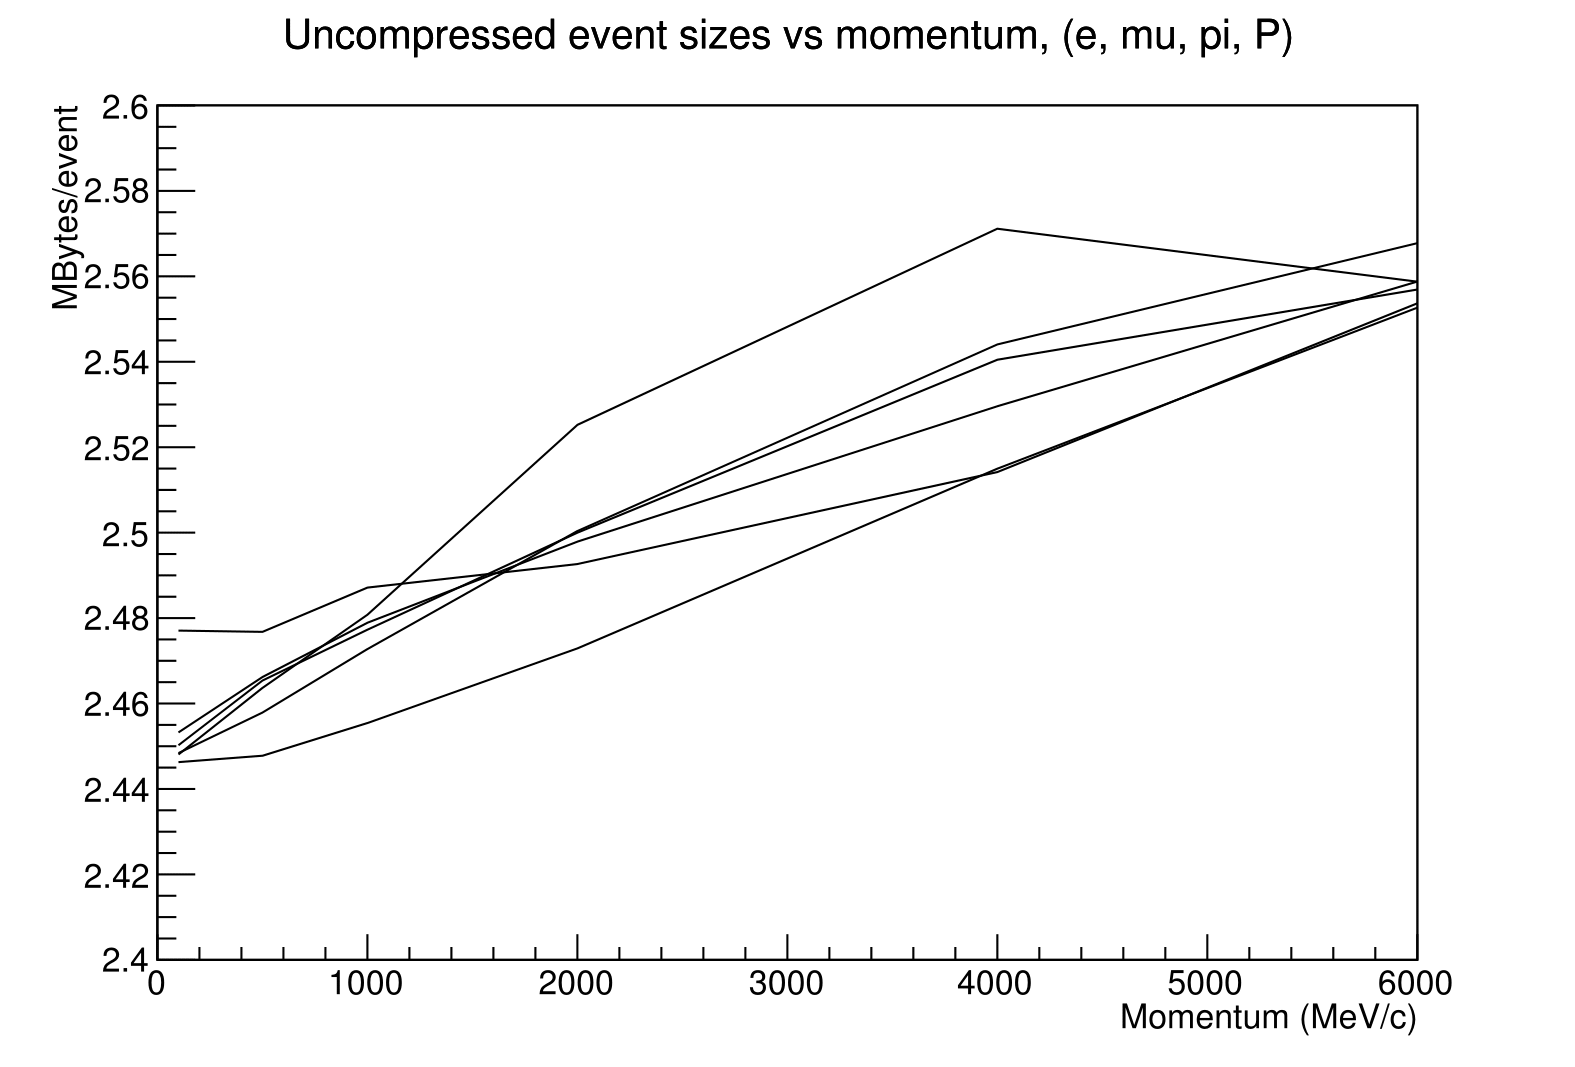
\includegraphics[width=0.6\textwidth]{btot.png}
	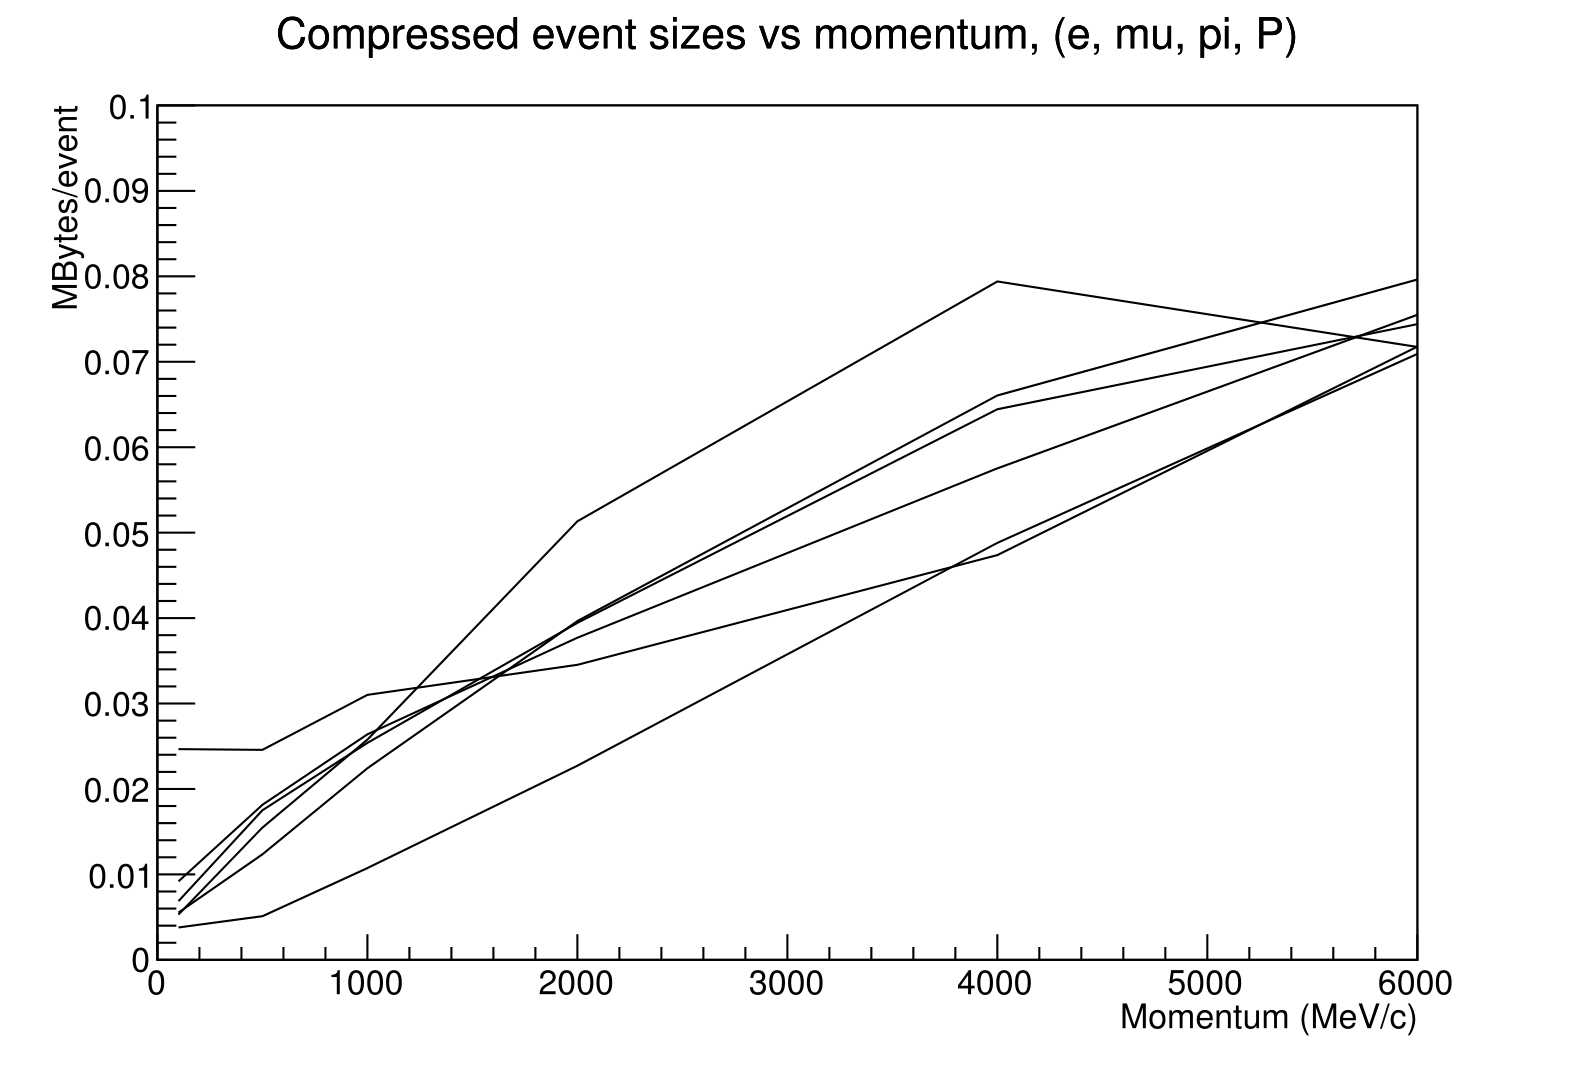
\includegraphics[width=0.6\textwidth]{bzip.png}
	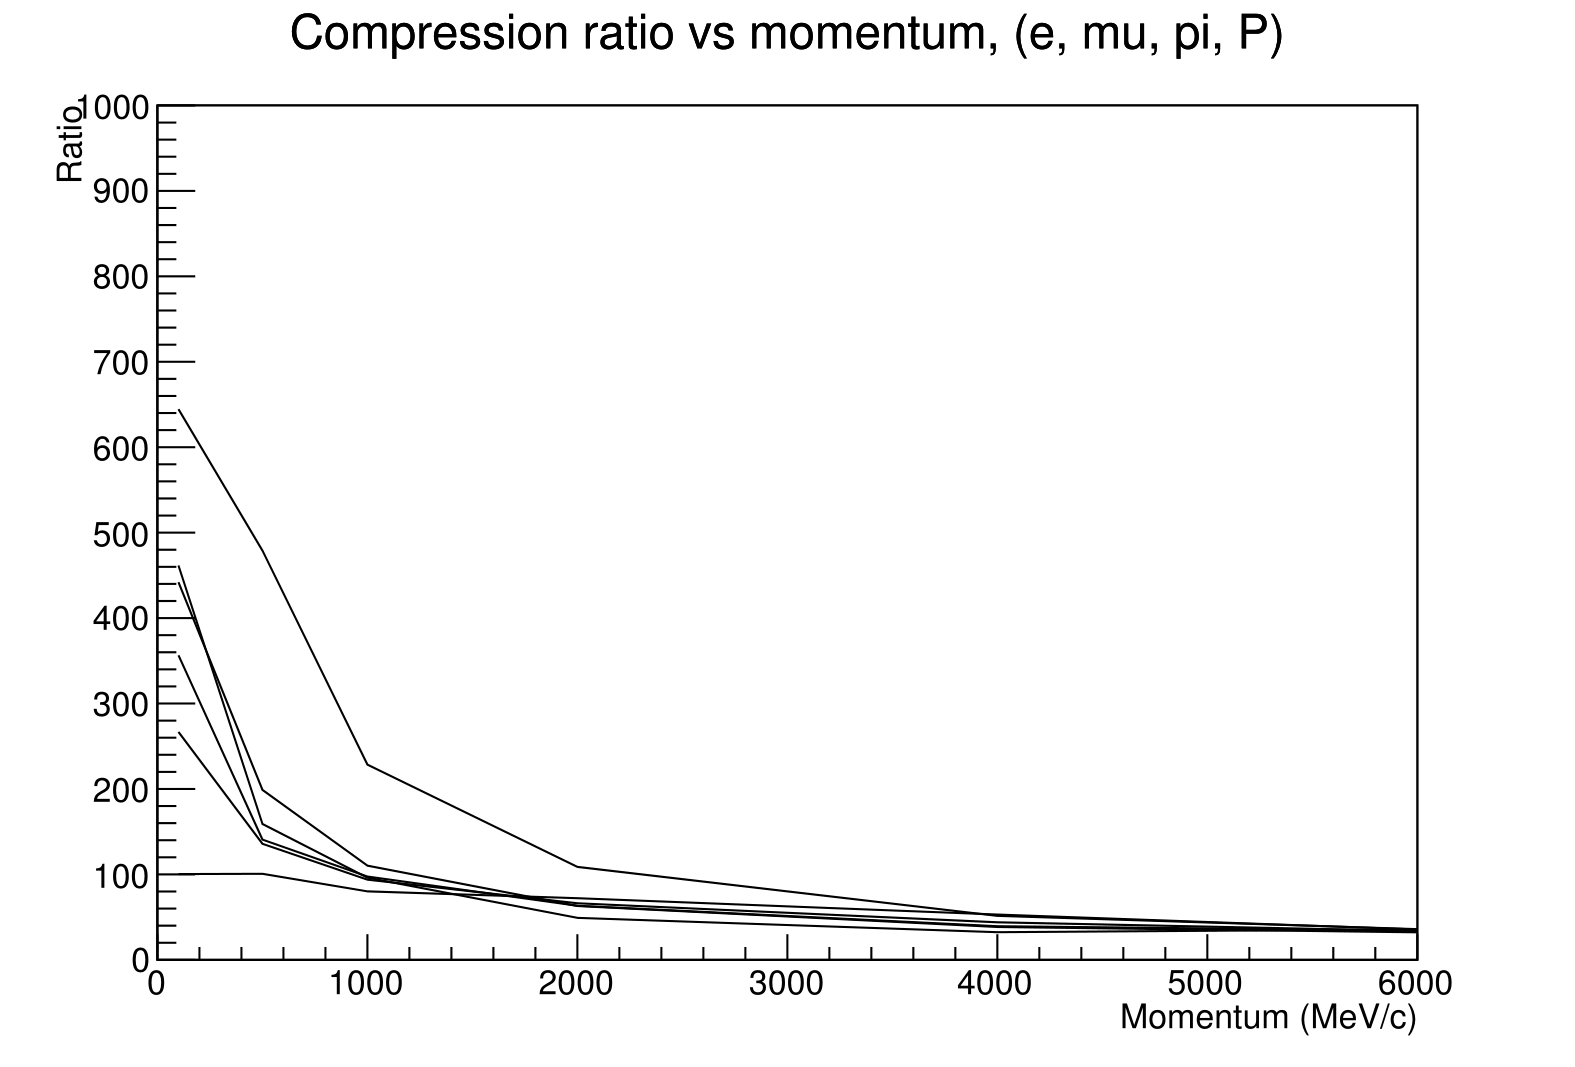
\includegraphics[width=0.6\textwidth]{brat.png}
	\caption{Estimation of DUNE zero-suppressed event sizes for different particles and momenta before and after compression, and their ratios.}
	\label{fig:data-compression}
\end{figure}
In order to estimate the effects of compression, specific particle types and energies were simulated using LArSoft.
The initial kinematics for the simulated samples covered a matrix of
particles ($e$, $\mu$, $\tau$, $\pi^+$, $\pi^-$, $\pi^0$ and proton) and momenta
(100\,MeV to 6\,GeV). The uncompressed and compressed sizes are summarized in Fig.~\ref{fig:data-compression}.

This exercise discovered a few types of inefficiencies in the design of data structures
currently used, which is unsurprising given that the DUNE software is undergoing active development
and not every optimization could be done until now. In one example, the bulk of the
compressed data written by LArSoft is actually made up channel ID
numbers providing a data inflation of about a factor of 10.
For uncompressed data this added about 50\%.
There are also additional data elements which are likely superfluous or
repeated more frequently than is likely to be required.
For example, in some types of the LArSoft output, even though zero suppression is applied, every
channel has an associated a pedestal and a sigma. There are other bits of superfluous data, but
they are not included in Fig.~\ref{fig:data-compression}. From the data presented in these
plots, the change in uncompressed event size is only a minor function of event momenta and
particle types. This is likely to be due to LArSoft saving additional overhead for all
channels, even those that have been fully zero-suppressed.

The simulation used to create these estimated included a detector module with
300,000 wires. The fact that the channel count in the full reference detector is
some 5 times larger will not change these estimates by a considerable margin
since it is assumed that DAQ/online systems will be capable of
not only of zero-suppression and compression, but also of suppression
of diffuse radiological backgrounds (see~\ref{sec:daq-assumptions}).
In other words, under normal conditions a cosmic $\mu$ or a beam
neutrino interaction will result in a localized ionization pattern (which
however may include long tracks) and the resulting data will not
scale linearly with the total channel count of the detector (which
sill still be effectively ``empty'' after suppression of $^{39}$Ar
background).

We then select the uncompressed event size to be 2.5\,MB and
the compressed event size of 0.2\,MB based
on data presented in Fig.~\ref{fig:data-compression} and
introducing a ``safety factor'' of 2 since the exact performance
of the data structures used in the final detactor cannot be precisely predicted at this time.

\subsubsection{High-Threshold data volume summary (revised)}
\label{sec:fd-data-volume-summary}
Taking into account arguments presented above, and uncertainties of up to factor of 3 in the Zero Suppression
performance to be realized in the final system (see~\ref{sec:zs-data}), we summarize data volume estimate for
the high energy domain in Table~\ref{tab:fd-data-volume-summary}.
\begin{table}[ht!]
\centering
\begin{tabular}{| p{1.5in} | p{0.95in} | p{0.75in} | p{0.8in} | p{0.9in} |}		\hline	
Source & Event Rate & Event Size & Data Rate & Volume/year \\ \hline
cosmic-$\mu$ & 0.259Hz & 0.6\,MB & 155.4\,kB/s & 4.8\,TB \\ \hline
beam-$\nu$ & 8770 year$^{-1}$ & 0.6\,MB & 0.17 kB/s & 5.3\,GB \\ \hline
Nucleon Decay cand. & - & 0.6\,MB & - & 480\,GB \\ \hline
\end{tabular}
\caption{Revised data rate and volume estimations for the High-Energy threshold.}
\label{tab:fd-data-volume-summary}
\end{table}



\subsection{The Near Detector Data}
\label{sec:nds-event-rates}
At the time of writing, there are many parameters of the NDS (see~\ref{sec:nds-params})
that are yet to be well defined. One set of parameters being considered at the time of writing is presented in
Table~\ref{tab:nds-params}. Table~\ref{tab:nds-event-rates} summarizes current estimates of the event rates
in the ND systems from various sources.

\begin{table}[ht!]
\centering
\begin{tabular}{| p{0.8in} | p{0.8in} |}		\hline		
\textbf{Source} & \textbf{Rate} (Hz)\\ \hline
Beam-$\nu$ & 40.2 \\ \hline
Rock & 10.0 \\ \hline
Cosmic & 0.04 \\ \hline
Total & 50.2 \\ \hline
\end{tabular}
\caption{Summary of combined DUNE Near Detector system event rate estimations.}
\label{tab:nds-event-rates}
\end{table}

\noindent
The projected data rate from the NDS is based on these event rates and occupancy estimated in preliminary Monte Carlo Studies,
and estimated number of samples to be read out per trigger ($\sim$4000). Preliminary size of each sample is 5B, resulting in an estimate
of $O(1)$\,MB per second data rate from the NDS. It is stated conservatively that the annual NDS data volume will be up to 100\,TB.
More information will be added to these estimates as the R\&D in this area progresses.
%\fxnote{More development needed here and more information from the ND people}

\subsection{Treatement of the Near Detector vs the Far Detector Data}
\label{sec:near-vs-far-data}
There is a small but important detail concerning how the ND and FD data streams are to be treated, and that is they are treated
separately i.e. not merged into common files.  This is due to the fact that these detectors are effectively looking at different sets
of events and there is no reason to complicate processing of the data by introducing such dependencies.

In general, they are also be processed in separate production streams and will require different and
distinct calibration procedures.

\subsection{Monte Carlo Data}
\label{sec:mc-data-estimates}
\subsubsection{Overview}
DUNE makes extensive use of Monte Carlo (MC) Simulations to optimize it multiple components and subsystems and is as an enabling factor in its physics
analysis. This area is an essential part of the Computing Model and issues related to characteristics of the Monte Carlo data must be addressed.
The following simulation areas are of particular interest:
\begin{itemize}
\item Beamline and Target simulations
\item Far Detector characterization
\item Near Detector Systems R\&D
\end{itemize}

\noindent
In addition to the above, DUNE must provide the necessary MC support for its vigorous prototyping program such as for the 35t detector
at FNAL and protoDUNE at CERN (see Sec.~\ref{sec:dune-prototypes} for more details), and this activity is largely aligned with the Far
Detector simulations.

In this section the focus is on quantifying the parameters of the data and the requisite CPU requirements will be considered separately.

\subsubsection{Beamline and target MC}
Optimization of the neutrino beam to be produced at LBNF for DUNE is absolutely essential for the scientific objectives of the experiment
to be achieved~\cite{cdr_vol2}. Detailed description of this work area is outside of the scope of this document. This work includes
optimization of the proton beam, target, focusing system, decay pipe and other components, and involve more than one software suite,
i.e. GEANT4~\cite{geant4} as well as MARS~\cite{mars}.

While the CPU requirements (analyzed separately) are quite substantial for this type of simulations, the amount of data to be managed
and committed to storage is not. There are two or three distinct simulations campaigns annually (with different versions of software),
each using O(100GB) of mass storage, so at the time of writing the scale is 1\,TB of data or less annually, based on bookkeeping records.

\subsubsection{Far Detector MC}
Far Detector simulations are done with multiple goals in mind. For example, the choice of wire plane geometry, e.g. the parameters of the wire
pitch, need to be evaluated and their effect on the detector performance quantified. Event recontruction in DUNE is a challenge (see
Appendix section~\ref{sec:reconstruction}) and detailed simulations are needed to estimate various efficiencies and other aspects
of the detector performance with respect to a variety physics processes.

MC event sizes vary depending on the conditions of the simulation, but on average are estimated to be $\sim$7\,MB per event
with the software configuration used at the time of writing. Current scale of data produced during a single Monte Carlo
campaign is $\sim$2.5\,TB. In a course of a year, roughly six MC campaigns are expected to take place, with resulting data volume of $\sim$15\,TB per year.

\subsubsection{Near Detector MC}
Final technology choices for some core elements of the Near Detector are yet to be made. Estimates show that event sizes will be similar
for two TPC options being considered: Liquid Argon TPC and gas-based TPC, and they both are in the range of $\sim$5\,MB per event.
With anticipated three campaigns every four months and ballpark statistics similar to that of the Far Detector simulation campaigns,
annual volume of data is $\sim$20\,TB.

\subsubsection{Other types of Monte Carlo}
In addition to the types of Monte Carlo simulations discussed above, there are occasionally studies in other subject areas,
such as estimating cosmic-ray induced backgrounds to nucleon decay and others. Once again, while doing these calculations
may require substantial CPU resources, the logic of the application is typically such that most of event selection takes place
in the application itself, limiting the resulting data volume and requisite storage space. 

\subsubsection{Summary of the MC data volume from different sources}
Estimates provided here are based on actual resource utilization over a few months at the time of writing, and are subject
to change. Types and volume of data generated in the course of DUNE Monte Carlo studies are summarized in Table~\ref{tab:mc-data}.
\begin{table}[ht!]
\centering
\begin{tabular}{| p{1.8in} | p{2.1in} |}		\hline		
\textbf{Type/Source} & \textbf{Annual Data Volume, TB}\\ \hline
Beamline and Target & 1 \\ \hline
Far Detector & 15 \\ \hline
Near Detector & 20 \\ \hline
Others & <1 \\ \hline
\end{tabular}
\caption{Summary of Monte Carlo Data Volume Estimates in DUNE.}
\label{tab:mc-data}
\end{table}

\subsection{Derived Data}
\label{sec:derived-data}
\subsubsection{Types of Data}
According to definition given in \ref{sec:req-data-definitions}, ``processed'' data includes the Monte Carlo data and
also data derived from either raw data or Monte Carlo, such as reconstructed event elements and physics-type objects
in any stage of processing.

At the time of writing, the reconstruction chain in DUNE and data formats for its implementation are in initial
stages of development, therefore in order to be able to produce estimates it is necessary to analyze and extrapolate
data models and formats used in contemporary large-scale experiments (e.g. the LHC). In doing so, the following elements
and formats of the derived data are observed to be in common in a few experiments:

\begin{itemize}

\item ESD (Event Summary Data): an object representation which contains the detailed output of the detector reconstruction and is
produced from the raw data.

\item AOD (Analysis Object Data): an object representation which contains a summary of the reconstructed event,
and contains sufficient information for common analyses.

\item DPD (Derived Physics Data): reductions of the AOD specific for particular types of analysis.

\end{itemize}

\noindent
There are sometimes additional formats of data defined for specific aspects of the Monte Carlo simulation studies, such as
event generator output, ``hits'' and others, but at present stage such level of detail in dealing with MC in DUNE is not
justified by practical considerations, and current estimates are based on ``bulk'' file size and scale of Monte Carlo campaigns.

Using this classification it is possible to extrapolate from the scaling of the event size observed at the LHC as the data
is undergoing transformations in the reconstruction and analysis chain. It is estimated that the ESD event size will be
$\sim$1.5\,times larger that the raw data, while AOD will be a fraction of $\sim$0.2 of the ESD and thus $\sim$0.3 fraction
of the raw data.
% NB. -mxp-
%ATLAS: ESD -- factor of 3 over raw, AOD -- 10 percent of ESD
%CMS:    ESD -- factor of 2 over raw, AOD -- 30 percent
A factor of 1.8 can be therefore used as the initial and very coarse estimate of the ratio of derived data volume to
the original raw data, which is appropriate to round up to 2.0.

Regarding the DPD segment of the derived data, no estimates can be provided at this point but it's fair to say that since
its creation involves a variety of reduction techniques (``skimming'', ``thinning'' etc) the resulting volume will be smaller than
the AOD. For this reason, contribution from DPD is ignored and not included in these estimates.

\subsubsection{Headroom Factor}
An additional consideration must be given to the extremely likely scenario that same data (in any stage of
its transformation) may be processed more than one time, for example with two different software releases for comparison,
validation or other such reasons. Alternatively, same release maybe used in what it commonly termed ``reprocessing'',
which is based on new and/or better calibrations and possibly other configuration improvements. Note that this is entirely
distinct from the notion of replication which will be discussed separately. For efficiency of operations (e.g. minimizing copy
to and from tape due to insufficient disk space) it is necessary to assume a certain ``headroom'' factor which would allow
for a few (not necessarily many) versions of the derived data to be disk-resident (including being available via
network access). While at this stage in the development of DUNE it is impossible to assign any precise number to this
factor, an assumption will be made that it is 4, such as to allow reprocessing of a sample of raw data by two separate
software releases.

\subsubsection{Summary}
\label{sec:derived-data-factor}
A few assumptions have been made regarding the total size of the derived data with respect to the raw data. By counting
different types and scales of the derived data coarsely based on the LHC experience, a factor of 2 over the raw data can
be deduced. A further factor of 4 may be necesary to allow for ample space during production with more than version
of software release and calibration data, for optimal efficiency. In summary, it is assumed for purposes of current estimates
that a total factor of 8 needs to be applied to the size of raw data to give the ballpark value of storage requirements for
the derived data.

